\section{Motivación e identificación del problema}
Un artículo wiki puede llegar a tener miles de ediciones a través del tiempo, en donde cada edición tiene la fecha y hora, el nombre de usuario o dirección de IP, el tamaño de la página en bytes, la diferencia de tamaño de página entre la edición y el estado anterior, una pequeño texto resumiendo la edición, entre otros atributos. Sin embargo, a simple vista todos estos datos pueden ser difíciles de leer y comprender por un humano, planteado esto surge la iniciativa de proyectar los datos a través de gráficas, lo que sería visualización de datos, en donde es posible ofrecer una información más clara y simple, además de poder explorar y hacer comparaciones entre los datos y el tiempo de manera visual para poder obtener una información más interesante al respecto.

\section{Objetivos del trabajo}
\subsection{Objetivo General}
Desarrollar una aplicación web que permita construir y editar visualizaciones de propiedades de historiales de wikis.
\subsection{Objetivos Específicos}
\begin{itemize}
\item Diseñar visualizaciones generales basadas en la información de los historiales de artículos de wikis provista por el API de Wikimetrics 2.0.
\item Definir los requerimientos de la aplicación.
\item Implementar una interfaz SPA adaptativa que ofrezca las funcionalidades requeridas por un \textit{watcher} de un wiki.
\item Utilizar un método ágil para el desarrollo de la aplicación.
\item Realizar el despliegue y puesta en producción.
\end{itemize}

\section{Estrategia de solución y método de desarrollo ágil a utilizar}
Los objetivos específicos serán desglosados de manera técnica en pequeñas tareas ordenadas por prioridad. El control de estas asignaciones se manejará mediante la plataforma GitHub (aplicación web para alojar repositorios Git) en donde cada tarea será un \textit{issue} a resolver. Github nos permite proyectar estos \textit{issues} en una pizarra, con el fin de visualizar el estado de cada asignación, los estados definidos son: Por hacer, En progreso, Terminado. Puede verse un ejemplo en la \textbf{Figura \ref{fig:githubBoard}}

\begin{itemize}
\item\textbf{Por hacer:} representa aquellas tareas especificadas, que por el momentos son \textit{issues} sin resolver.
\item\textbf{En progreso:} representa las tareas que están siendo desarrolladas, cabe destacar que cada asignación se resuelve en una rama distinta del repositorio git haciendo uso del \textit{pull request} para llevar un mayor control del desarrollo de la asignación.
\item\textbf{Terminado:} representa aquellas tareas culminadas. Cuando se considera que una tarea está lista, esta tiene que ser mezclada a la rama principal del repositorio, llamada \textit{master}, luego cerrar el \textit{pull request} y el \textit{issue} asociado.
\end{itemize}
\bigbreak
\begin{center}
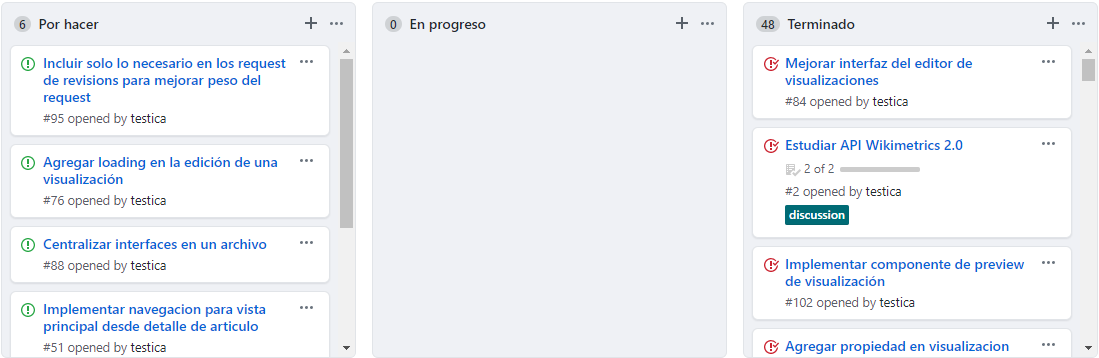
\includegraphics[scale=0.5]{github_board.png}
\captionof{figure}{Ejemplo de pizarra de Github}
\label{fig:githubBoard}
\end{center}
\bigbreak
La pizarra de Github manifiesta una metodología Kanban \cite{BookKanban}, en donde visualizar el flujo de trabajo y hacerlo visible es la base para comprender cómo avanza el trabajo. Sin comprender el flujo de trabajo, realizar los cambios adecuados es más difícil. Una forma común de visualizar el flujo de trabajo es el uso de columnas. Las columnas representan los diferentes estados o pasos en el flujo de trabajo. Kanban logra un desarrollo evolutivo e incremental, donde las soluciones de las asignaciones puede que no sean las mejores comenzando, pero a medida que se itera se va perfeccionando.

\section{Trabajos similares, diferencias y ventajas de la solución a desarrollar}
Wikimedia Tools Labs\footnote{Wikimedia Tool Labs \url{https://tools.wmflabs.org/}} es una página que ofrece un ambiente apropiado para los desarrolladores de la comunidad, en donde podemos encontrar una lista de herramientas elaboradas por personas que trabajan sobre wikis ayudando a facilitar determinadas tareas. Las siguientes herramientas son similares:
\begin{itemize}
\item\textbf{WikiHistory}\footnote{WikiHistory \url{https://tools.wmflabs.org/xtools/wikihistory/}}:
Esta herramienta web, nos ofrece para cada wiki, una información general, en donde podemos saber cuántos usuarios editan por día, al mes o al año, la primera y última edición, entre otras cosa como se puede observar en la \textbf{Figura \ref{fig:wiki_history1}}. En la misma sección de información general es proyectada una gráfica de porcentajes sobre el tipo de edición, véase la \textbf{Figura \ref{fig:wiki_history2}}. También nos ofrece una gráfica de Línea de Tiempo, vea \textbf{Figura \ref{fig:wiki_history3}}, en donde podemos saber la cantidad de ediciones filtradas por año, mes o semana. Por último brinda una tabla de los usuarios que han editados, tomando en cuenta la cantidad de ediciones y la fecha de la primera y última edición. 
\bigbreak
\begin{center}
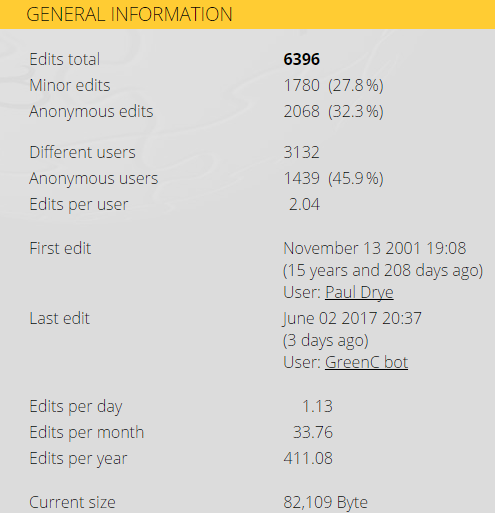
\includegraphics[scale=0.55]{wiki_history1.png}
\captionof{figure}{Información general proporcionada por la herramienta WikiHistory sobre el artículo 'Chocolate'.}
\label{fig:wiki_history1}
\end{center}
\bigbreak
\begin{center}
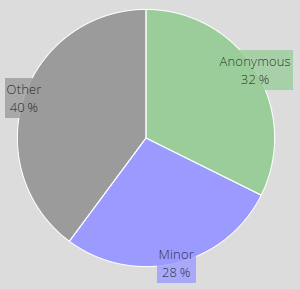
\includegraphics[scale=0.70]{wiki_history2.png}
\captionof{figure}{Gráfica de tipo torta de WikiHistory, que refleja el porcentaje de ediciones anónimas, menores y otras, sobre el artículo 'Chocolate'.}
\label{fig:wiki_history2}
\end{center}
\bigbreak
\begin{center}
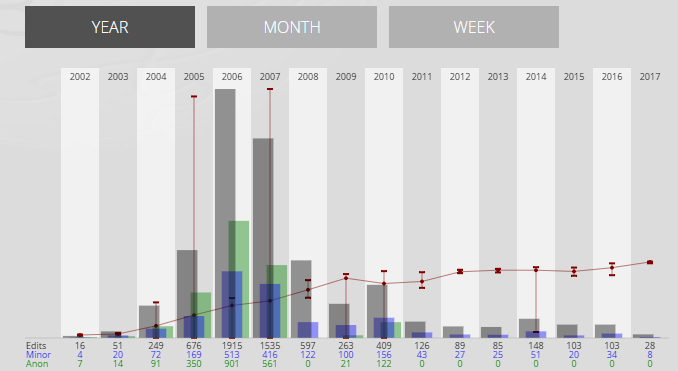
\includegraphics[scale=0.40]{wiki_history3.png}
\captionof{figure}{Línea de tiempo, que proyecta visualmente las ediciones totales, menores y anónimas del artículo 'Chocolate', que pueden ser filtradas por año, mes o semana.}
\label{fig:wiki_history3}
\end{center}
\bigbreak
Esta página ofrece datos importantes pero de manera estática, es decir no podemos realizar otras consultas adicionales y solo ofrece dos (2) gráficas, nuestro trabajo explotará más el área de visualización de datos, dejando cierta libertad al usuario para que explore. Por otro lado, cuando el wiki tiene muchas ediciones de usuarios distintos la página tarda en cargar y se vuelve lenta debido a que el DOM tiene muchos elementos, la idea que nos llevamos a nuestro trabajo es mostrar la información por segmentos, ofreciendo paginación o filtros.

\item\textbf{PageViews}\footnote{PageViews \url{https://tools.wmflabs.org/pageviews/}}:
Es una herramienta para visualizar las vistas que ha recibido una wiki a través del tiempo, vea \textbf{Figura \ref{fig:page_views}}, lo interesante de esta herramienta es que podemos editar el intervalo de tiempo, además destaca la posibilidad de sobreponer las líneas de tiempo para poder comparar las visitas de varias wikis con el propósito de encontrar datos interesantes. Cabe acotar que nuestro trabajo no se especializará en visualizar las vistas de un wiki, pero esta herramienta logra exprimir el poder de la visualización de datos y eso es lo que queremos lograr pero con las propiedades de las ediciones de un wiki.
\bigbreak
\begin{center}
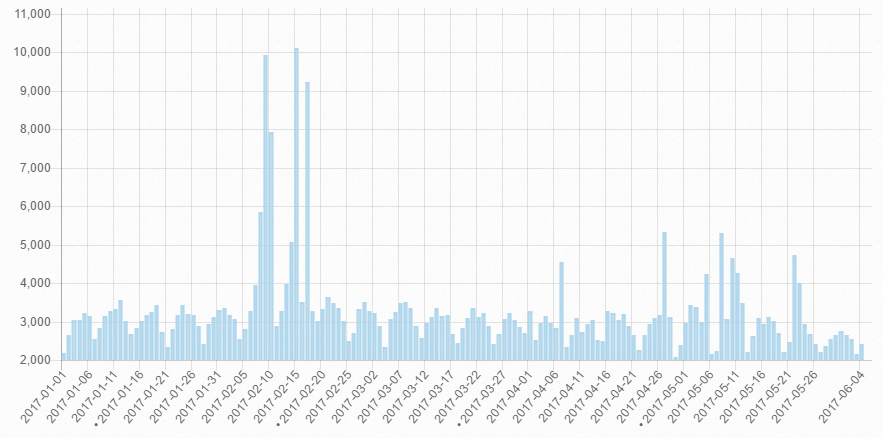
\includegraphics[scale=0.40]{page_views.png}
\captionof{figure}{Visualización tipo barra sobre el artículo 'Chocolate', en donde el eje 'y' representa el número de visitas, y el eje 'x' representa la fecha.}
\label{fig:page_views}
\end{center}
\bigbreak
\item\textbf{Chromograms} \cite{Chromogram}:
Es una técnica de visualización con el fin de encontrar patrones en las numerosas ediciones de un artículo de Wikipedia a través de colores. Chromogram corresponde un texto con un color, en donde las tres primeras letras de una palabra definen el color: la primera letra representa el matiz, la segunda la saturación y la tercera el brillo. Cada edición representa un rectángulo con un color posicionado de izquierda a derecha y de arriba hacia abajo. Podemos observar un ejemplo en la \textbf{Figura \ref{fig:chromogram}}
\bigbreak
\begin{center}
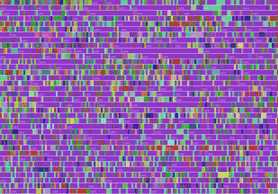
\includegraphics[scale=0.80]{chromograms.png}
\captionof{figure}{Uso de Chromogram donde el color morado representa al artículo de US Ships (en donde el título del artículo empieza con 'USS')}
\label{fig:chromogram}
\end{center}
\bigbreak

\item\textbf{History Flow} \cite{HistoryFlow}:
Es una técnica de visualización que refleja el comportamiento de las ediciones en el tiempo según el usuario que la realizó. Como indica la \textbf{Figura \ref{fig:historyFlow1}}, cada edición es representada mediante una barra vertical en donde cada porción de color en la barra representa el usuario, cabe destacar que cada usuario tiene un color específico. Esta visualización nos reporta el crecimiento en el tiempo del artículo wiki, y gracias a los colores podemos observar patrones e identificar comportamientos sospechosos como lo muestra la \textbf{Figura \ref{fig:historyFlow2}}.
\bigbreak
\begin{center}
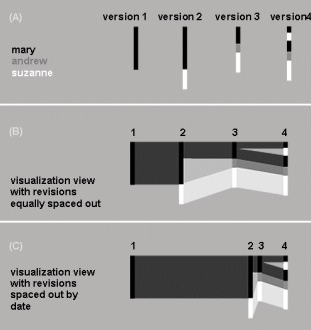
\includegraphics[scale=0.80]{history_flow1.png}
\captionof{figure}{Explicación del mecanismo de visualización de History Flow}
\label{fig:historyFlow1}
\end{center}
\bigbreak
\begin{center}
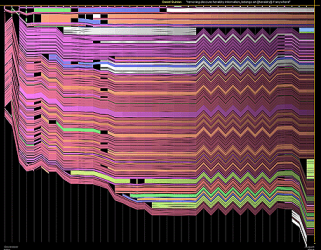
\includegraphics[scale=0.80]{history_flow2.png}
\captionof{figure}{En la página 'Chocolate' se observa un patrón en zigzag que demuestra una guerra de ediciones}
\label{fig:historyFlow2}
\end{center}
\bigbreak
\item\textbf{History Graph} \cite{HistoryGraph}:
Es una adaptación de la técnica de visualización \textit{History Flow}, donde cada barra de la visualización corresponde a una versión, el ancho de cada barra corresponde a la distancia con respecto al cambio anterior, el alto de la barra representa el tamaño en bytes de la versión y el color representa el usuario que hizo el cambio como se aprecia en la \textbf{Figura \ref{fig:historyGraph}}. Esta visualización es muy útil para proyectar la evolución en el tiempo de un artículo y observar la frecuencia de cambios, los usuarios que participan y el crecimiento/decrecimiento del texto editado.
\bigbreak
\begin{center}
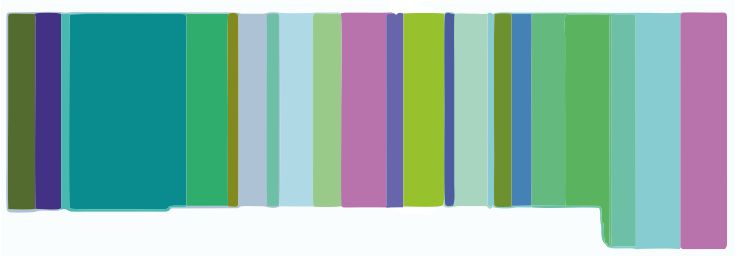
\includegraphics{history_graph.png}
\captionof{figure}{Demostración de History Graph}
\label{fig:historyGraph}
\end{center}
\bigbreak
\end{itemize}

\section{Herramientas}
\textbf{Tecnologías necesarias para el ambiente de desarrollo}
\begin{itemize}
\item Editor de texto inteligente (Visual Studio Code, Atom, Sublime Text, Notepad++, etc.)
\item Git, para manejar el versionamiento del código.
\item Navegador de Internet (Google Chrome o Firefox).
\item Alguna base de datos (preferiblemente MongoDB) para almacenar configuración de usuarios.
\item Servidor Web para levantar la aplicación (Node, Apache, etc.)
\\[5pt]
\end{itemize}

\textbf{Tecnologías web a utilizar}
\begin{itemize}
\item Bibliotecas de visualización: para las visualizaciones genéricas vamos a usar las bibliotecas \textbf{Echarts} y/o \textbf{Plotly}, para visualizaciones no comunes y que tengan una finalidad específica que puedan surgir usaremos \textbf{D3}.
\item Arquitectura: construiremos la aplicación con ayuda del framework \textbf{Angular 2}, que tiene un mayor enfoque SPA y logra una buena estructura en el código.
\item Diseño: con ayuda de la biblioteca \textbf{Angular Material} despliegaremos el diseño.
\item Biblioteca \textbf{Lodash} y \textbf{Moment} para facilitar ciertas tareas como el formato de fechas y manipulación de objetos y arreglos.
\\[5pt]
\end{itemize}

\section{Requerimientos}
\begin{itemize}
\item Una herramienta capaz de visualizar gráficas sobre propiedades de edición de un wiki.
\item Los wikis a visualizar son extraídas del watchlist del usuario autenticado a través de Wikipedia (usando API de MediaWiki).
\item Permitir editar las visualizaciones (alternar tipo de gráfica, cambiar los tipos de datos a visualizar).
\item Los datos a representar en las visualizaciones son proporcionados a través del API Wikimetrics 2.0.
\item La herramienta tiene que ser una aplicación web.
\item La aplicación tiene que contar con una vista principal que incluya gráfica e información general de cada uno de los wiki del watchlist.
\item Permitir al usuario crear una visualización nueva y guardarla de forma permanente, para este caso es necesario el uso de una base de datos (preferiblemente MongoDB)
\item La aplicación tiene que estar alojada en un servidor, para poder ser accedida de manera remota.
\\[5pt]
\end{itemize}

\section{Prototipo de interfaz}
\bigbreak
Como vista inicial, si no estamos autenticados, es el inicio de sesión, en donde hay que suministrar el usuario y contraseña de Wikipedia, vea \textbf{Figura \ref{fig:prototype_sign_in}}.
\bigbreak
\begin{center}
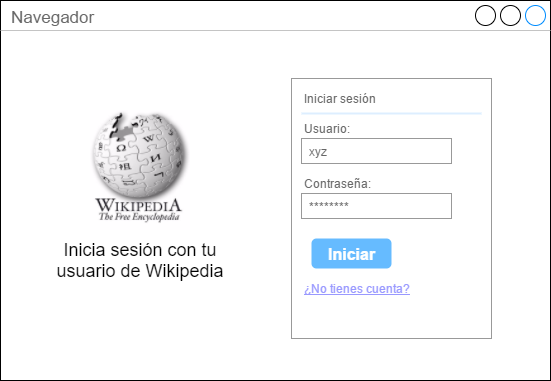
\includegraphics[scale=0.62]{prototype/sign_in.png}
\captionof{figure}{Interfaz para iniciar sesión}
\label{fig:prototype_sign_in}
\end{center}
\bigbreak
La vista principal, consta de un listado de los wiki del watchlist del usuario que inició sesión, con una visualización y un resumen general, vea \textbf{Figura \ref{fig:prototype_dashboard}}.
\bigbreak
\begin{center}
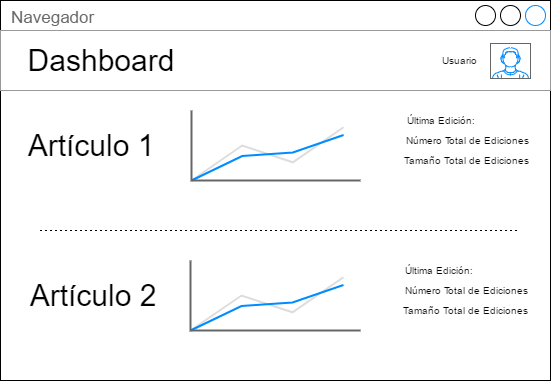
\includegraphics[scale=0.62]{prototype/dashboard.png}
\captionof{figure}{Interfaz de la vista principal}
\label{fig:prototype_dashboard}
\end{center}
\bigbreak
Al seleccionar uno de los wiki de la lista, accederemos a una vista detallada del mismo, en donde se ofrecerá información más específica y una lista de visualizaciones generales, adicionalmente un botón para poder crear una, vea \textbf{Figura \ref{fig:prototype_detail}}.
\bigbreak
\begin{center}
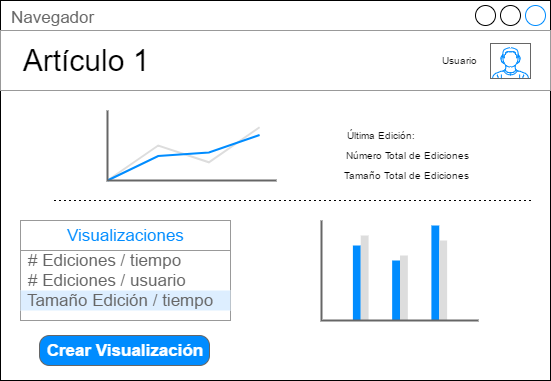
\includegraphics[scale=0.62]{prototype/detail.png}
\captionof{figure}{Interfaz de la vista detallada de un wiki}
\label{fig:prototype_detail}
\end{center}
\bigbreak
En la vista de creación de una visualización, es necesario suministrar un nombre y los ejes a comparar, de igual forma seleccionar el tipo de gráfica, vea \textbf{Figura \ref{fig:prototype_create}}.
\bigbreak
\begin{center}
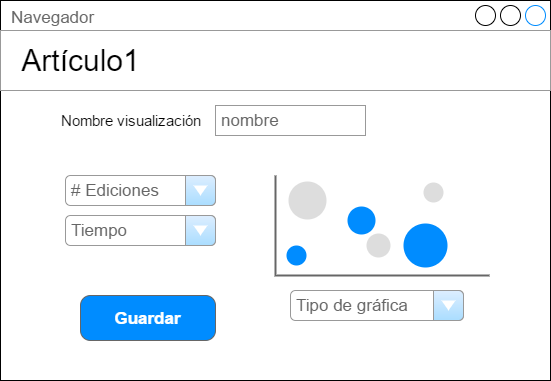
\includegraphics[scale=0.62]{prototype/create.png}
\captionof{figure}{Interfaz de la vista de creación de una visualización}
\label{fig:prototype_create}
\end{center}

\section{Planificación de las actividades}

\begin{tabular}{ |p{8cm}|p{4cm}|}
 \hline
 \textbf{Actividad} & \textbf{Tiempo estimado}\\
 \hline
 Preparar el entorno de desarrollo & 1/2 semana\\
 \hline
 Estudiar API Wikimetrics 2.0 (Back-end) & 1/2 semana\\
 \hline
 Estudiar API MediaWiki & 1/2 semana\\
 \hline
 Integración del API Wikimetrics 2.0 (Back-end) & 1/2 semana\\
 \hline
 Integración del API MediaWiki & 1/2 semana\\
 \hline
 Elaborar estructura base de la aplicación web & 1/4 semana\\
 \hline
 Definir que datos se van a almacenar del usuario e integrar base de datos & 1 semana\\
 \hline
 Implementar vista de iniciar sesión haciendo uso del API MediaWiki & 1/2 semana\\
 \hline
 Definir y diseñar gráficas generales en base a los datos que proporciona el API de Wikimetrics 2.0 & 2 semanas\\
 \hline
 Estudiar documentación de bibliotecas de visualización & 1 semana\\
 \hline
 Implementar vista de Dashboard & 1 semana\\
 \hline
 Implementar vista de Detalle de wiki, incluyendo gráficas generales & 2 semana\\
 \hline
 Diseñar e implementar creador de gráfica en base a los datos que proporciona el API de Wikimetrics 2.0 & 1 semana\\
 \hline
 Añadir estilo apropiado a la aplicación & 1/2 semana\\
 \hline
 Soportar adaptación a distintas pantallas & 1/2 semana\\
 \hline
 Añadir animaciones a la aplicación & 1/2 semana\\
 \hline
 Elaborar despliege de la aplicación & 1/2 semana\\
 \hline
\end{tabular}